\uuid{kT51}
\exo7id{5079}
\auteur{rouget}
\organisation{exo7}
\datecreate{2010-06-30}
\isIndication{false}
\isCorrection{true}
\chapitre{Nombres complexes}
\sousChapitre{Trigonométrie}

\contenu{
\texte{
Soit $k$ un réel distinct de $-1$ et de $1$.
}
\begin{enumerate}
    \item \question{Etudier les variations de $f_k~:~x\mapsto\frac{\sin x}{\sqrt{1-2k\cos x+k^2}}$.}
    \item \question{Calculer $\int_{0}^{\pi}f_k(x)\;dx$.}
\reponse{
\textbullet~Pour tout réel $x$, $1-2k\cos x+k^2=(k-\cos x)^2+\sin^2x\geq0$. De plus,

$$1-2k\cos x+k^2=0\Rightarrow k-\cos x=\sin x=0\Rightarrow x\in\pi\Zz\;\mbox{et}\;k=\cos x\Rightarrow k\in\{-1,1\},$$
ce qui est exclu. Donc,

$$\forall k\in\Rr\setminus\{-1,1\},\;\forall x\in\Rr,\;1-2k\cos x+k^2>0.$$
\textbullet$f_k$ est donc définie sur $\Rr$, dérivable sur $\Rr$ en vertu de théorèmes généraux, impaire et $2\pi$-périodique. On
l'étudie dorénavant sur $[0,\pi]$. Pour $x\in[0,\pi]$, on a~:

\begin{align*}
f'_k(x)&=\cos x(1-2k\cos x+k^2)^{-1/2}-\frac{1}{2}\sin x(2k\sin x)(1-2k\cos x+k^2)^{-3/2}\\
 &=(1-2k\cos x+k^2)^{-3/2}(\cos x(1-2k\cos x+k^2)-k\sin^2x)\\
 &=(1-2k\cos x+k^2)^{-3/2}(-k\cos^2x+(1+k^2)\cos x-k)\\
 &=(1-2k\cos x+k^2)^{-3/2}(k\cos x-1)(k-\cos x)
\end{align*}

\begin{center}
\shadowbox{
$\forall x\in\Rr,\;f_k'(x)=\frac{(k\cos x-1)(k-\cos x)}{(1-2k\cos x+k^2)^{3/2}}.$
}
\end{center}

\begin{itemize}
[\textbf{1er cas}~:~$|k|<1$ et $k\neq0$.] (si $k=0$, $f_k(x)=\sin x$) Pour tout réel $x$, $(1-2k\cos x+k^2)^{-3/2}(k\cos
x-1)<0$ et $f_k'(x)$ est du signe de $\cos x-k$.

$$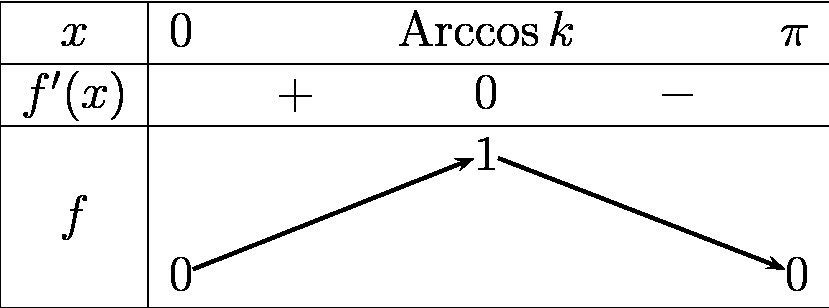
\includegraphics{../images/img005079-1}$$

(car $f_k(\Arccos k)=\frac{\sqrt{1-k^2}}{\sqrt{1-2k^2+k^2}}=1$).
[\textbf{2ème cas}~:~$k>1$.] Pour tout réel $x$, $(1-2k\cos x+k^2)^{-3/2}(k-\cos x)>0$ et $f_k'(x)$ est du signe de $k\cos
x-1$.

$$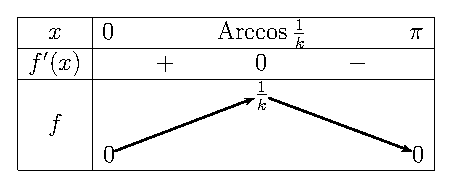
\includegraphics{../images/img005079-2}$$

(car $f_k(\Arccos\frac{1}{k})=\frac{\sqrt{1-\frac{1}{k^2}}}{\sqrt{1-2+k^2}}=\frac{1}{k}$).
[\textbf{3ème cas}~:~$k<-1$.] Pour tout réel $x$, $(1-2k\cos x+k^2)^{-3/2}(k-\cos x)<0$ et $f_k'(x)$ est du signe de
$1-k\cos x$.

$$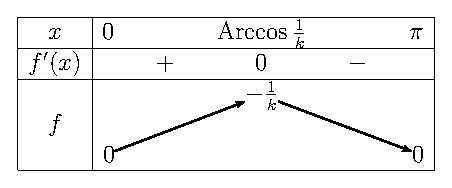
\includegraphics{../images/img005079-3}$$



(car $f_k(\Arccos\frac{1}{k})=\frac{\sqrt{1-\frac{1}{k^2}}}{\sqrt{1-2+k^2}}=-\frac{1}{k}$).

\end{itemize}
Pour $k\in\Rr\setminus\{-1,1\}$, posons $I_k=\int_{0}^{\pi}f_k(x)\;dx$.

Si $k=0$, $I_k=\int_{0}^{\pi}\sin x\;dx=2$. Sinon,

\begin{align*}
I_k&=\frac{1}{k}\int_{0}^{\pi}\frac{2k\sin x}{2\sqrt{1-2k\cos x+k^2}}\;dx=\frac{1}{k}
\left[\sqrt{1-2k\cos x+k^2}\right]_0^\pi\\
 &=\frac{1}{k}(\sqrt{1+2k+k^2}-\sqrt{1-2k+k^2})=\frac{1}{k}(|k+1|-|k-1|).
\end{align*}
Plus précisément, si $k\in]-1,1[\setminus\{0\}$, $I_k=\frac{1}{k}((1+k)-(1-k))=2$, ce qui reste vrai pour $k=0$. Si
$k>1$, $I_k=\frac{1}{k}((1+k)-(k-1))=\frac{2}{k}$, et enfin, si $k<-1$, $I_k=\frac{-2}{k}$. En résumé,

\begin{center}
\shadowbox{
$\mbox{Si}\;k\in]-1,1[,\;I_k=2\;\mbox{et si}\;k\in]-\infty,-1[\cup]1,+\infty[,\;I_k=\frac{2}{|k|}.$
}
\end{center}
}
\end{enumerate}
}
